\documentclass{article}
\usepackage[a4paper, total={6in, 8in}]{geometry}
%\usepackage{cite}
\usepackage{titlesec}
\usepackage{amsmath}
\usepackage{caption}
\usepackage{graphicx}
\usepackage{float}
\usepackage{matlab-prettifier}
\usepackage[sorting=none, backend=biber, style=ieee]{biblatex} 
\addbibresource{Thesis.bib}
\setcounter{secnumdepth}{4}

\makeatletter
\def\input@path{"./MATLAB Software"}
\makeatother

\graphicspath{{./figures/}}
\graphicspath{{./images/}}
\allowdisplaybreaks
\title{Data Analysis for Predictive Maintenance of a Straightening Machine in the Steel Industry}
\date{2023-09-XX}
\author{Paul Barron}
\begin{document}
\pagenumbering{gobble}
\maketitle
\newpage
\pagenumbering{arabic}
\tableofcontents
\newpage
\section{Abstract}
Large large machinery is expensive to run and downtime can be very costly. There is a large area of work dedicated to analyzing the health of a machine, predicting the remaining life and time to failure.
\clearpage
\section{Acknowledgments}
\clearpage
\section{Introduction}
\subsection{Background}
%Discuss why condition monitoring is important
The subject of condition monitoring and predictive maintenance is a large area of research in the machine and manufacturing world. Extracting condition indicators in order to monitor equipment health and predict remaining lifetime can have valuable benefits to any company. Avoiding unplanned downtime and catastrophic failure allows the extraction of more value from resources already in place and thus financial benefits.

%What is condition monitoring
Condition monitoring describes of a set of sensors that measure physical conditions of a machine such vibration, temperature, acoustics etc. in addition to an algorithm that takes the sensor data as input and outputs a health metric.

Advanced monitoring of machining operations~\cite{teti2010advanced}

Not only machines but other engineering structures like bridges and also in biological systems.

%Discuss more specifically bearing vibration analysis
A common application of condition monitoring is the vibration analysis of rotating machines. The degradation of a bearing results changes in the vibration signal which can be a indicator of bearing health. ~\cite{soualhi2021novel}.
[A Review on Vibration-Based Condition Monitoring of Rotating Machinery]
%Even more specifically a tube straightening machine
One such example of an industrial machine that uses roller bearings is a rotary tube straightening machine. These are used in the steel industry for the manufacturing of steel tubes. They are crucial for straightening the tube in the longitudinal direction and improving roundness of the product~\cite{yoshimura2009effect}. Significant research exists on the mechanical analysis of such machines ~\cite{kato2014straightening}~\cite{ma2020effect}~\cite{ma2021analysis}~\cite{yu2018theoretical}~\cite{das1991mechanics}. 

%Explain why condition monitoring would be useful for a straightening machine
Such machines expensive to build and/or acquire and down time can be costly. Performance may also be impacted by the machine being in poor condition requiring maintenance. Thus it is in the interest of the operators to be able to assess the machine condition, predict the remaining useful life and prevent unplanned downtime and catastrophic failures.

%Difficult to obtain failure data
"Because slewing bearing is a large low-speed heavy-load bearing, vibration signal is insufficient. On the other hand, because of the influence of the
environment, it is difficult to obtain failure data of slewing bearing under actual working conditions, and tests also will entails high costs, so that the failure data is limit."This paper discusses a life forcasting model~\cite{wang2016multiple}

\begin{figure}[H]
	\centering
	\includegraphics[width=90mm, keepaspectratio]{straightening2.png}
	\caption{A straightening machine~\cite{ma2020effect}}
	\label{straighteningImage2}
\end{figure}

\begin{figure}[H]
	\centering
	\includegraphics[]{straightening1.jpg}
	\caption{A straightening machine~\cite{kato2014straightening}}
	\label{straighteningImage1}
\end{figure}

\begin{figure}[H]
	\centering
	\includegraphics[]{straightening3.jpg}
	\caption{A straightening machine~\cite{ma2021analysis}}
	\label{straighteningImage3}
\end{figure}

\begin{figure}[H]
	\centering
	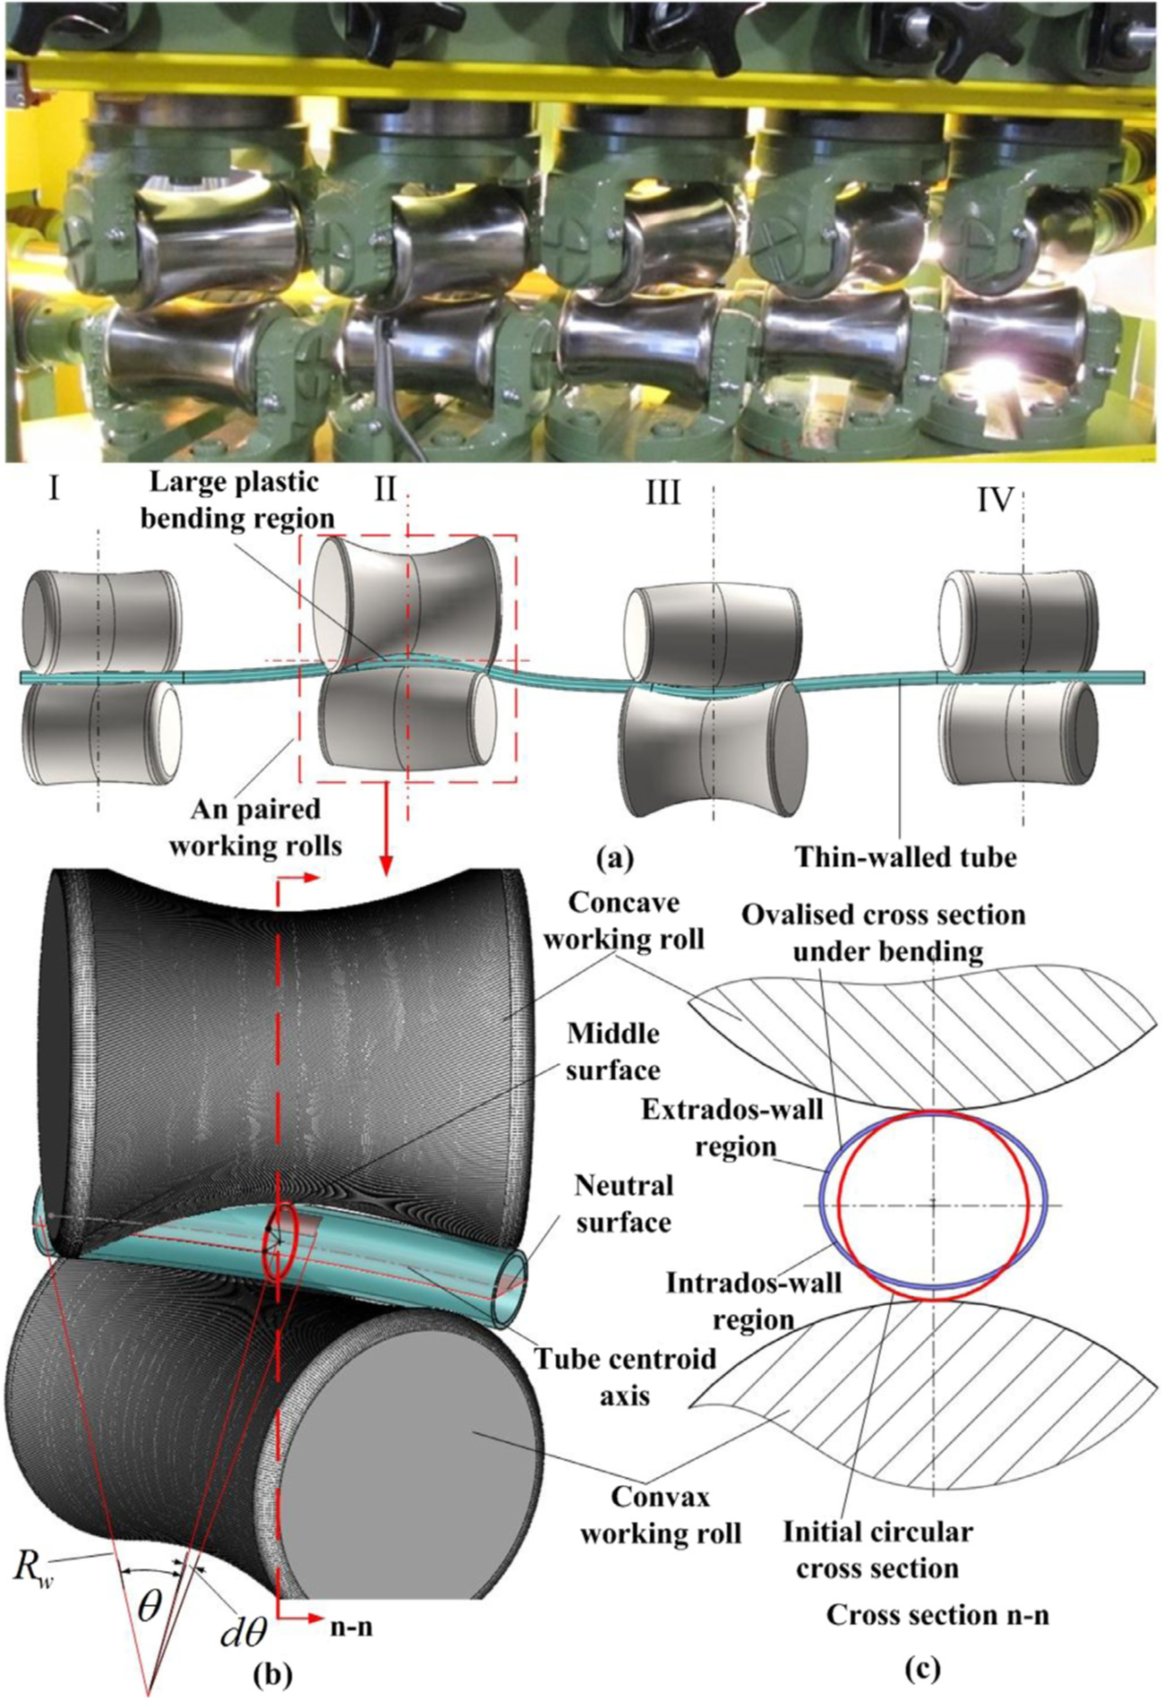
\includegraphics[width=90mm, keepaspectratio]{Straightening5.png}
	\caption{A straightening machine~\cite{zhang2019modeling}}
	\label{straighteningImage5}
\end{figure}

\subsection{Project Aim}
The aim of this project is to examine the existing data collection strategy for a tube straightening machine and make some suggestions as to whether it is possible to perform condition monitoring and/or remaining life analysis for this machine. The first step analyze the available data that can be be attained using the existing sensors and data acquisition system. The end foal is to begin developing a strategy that will assist the company to know when the machine requires maintenance. The specific goals of this project are summarized as follows:
\begin{itemize}
\item Understand what signals are related to each other.
\item Understand the signals from a statistical point of view.
\item Identify which features are of significance and which are not useful for condition monitoring i.e. which features may represent degradation condition.
\end{itemize}
%\subsection{Tools}
%MATLAB Diagnostic Feature Designer.
%\subsection{Structure of the Report}
\clearpage  
\section{Theory}
\subsection{Feature Extraction}
%Statistical learning?

%Feature Extraction in general
Feature extraction is the process of computing numerical values from raw data in order to reduce big data sets but preserves the information. Machine learning algorithms suffer from high volumes of data and information redundancy?

%Feature extraction used in condition monitoring/degradation
Feature extraction techniques for condition monitoring are used for estimating degradation trends~\cite{caesarendra2017review}~\cite{adams2017comparison}.

%Techniques for selecting features
This paper talks about "top sensitive features"~\cite{bleakie2013feature}.
This paper talks about defines feature goodness metrics of correlation (Corr), monotonicity (Mon) and robustness (Rob) ~\cite{zhang2016degradation}.

%Automatic feature extraction? Manual Feature extraction?
Acoustic emission signals. Ant colony optimization-based feature selection methods?~\cite{liao2010feature}.

This paper discusses a life forecasting model~\cite{wang2016multiple}
This PhD thesis does this..~\cite{martin2017unsupervised}

\subsection{Time Domain Features} 	
Features in the time domain. Statistical features, Impulsive Metrics, 
\subsubsection{Cross correlation}
\subsubsection{Mean}
The mean is simply the average value of the signal.
$$ \bar{x} = \frac{\sum^N_{i=i} x_i}{N} $$
\subsubsection{Standard Deviation}  
Measures the dispersion of a data set relative to its mean. Square root of variance.
$$ Var =\frac{\sum^N_{i=1}(x_i-m)^2}{(N-1)\sigma^2} $$
\subsubsection{Root Mean Square (RMS)}

$$ RMS = \sqrt{\frac{1}{N} \sum^N_{i=1}x^2_i} $$
\subsubsection{Shape Factor}

$$ \frac{ \sqrt{\frac{1}{N} \sum^N_{i=1}x_i^2} }  {\frac{1}{N}\sum^N_{i=1}|x_i|} $$
\subsubsection{Kurtosis}

$$ Ku = \frac{\sum^N_{i=1}(x_i-m)^4)}{(N-1)\sigma^4} $$ 
\subsubsection{Skewness} 
A measure of asymmetry of through probability density function.
$$ Sk = \frac{\sum^2_{i=1}(x_i-m)^3}{(N-1)\sigma^3} $$
\subsubsection{Peak Value}
Maximum vale of a signal
$$ PV = max(x_i) $$ 
\subsubsection{Impulse Factor} 
Impulse? Divides the maximum absolute value by the mean of absolute value
$$ x_{clear} = \frac{x_p}{(\frac{1}{N}\sum^N_{i=1}|x_i|)} $$  
\subsubsection{Crest Factor} 
Impact. Divide the maximum absolute value of vibration signal and
RMS value.
$$ CF = \frac{max|x_i|}{\sqrt{\frac{1}{N}}\sum^N_{i=1}x^2_i} $$
\subsubsection{Clearance Factor} 

$$ x_{clear} = \frac{x_p}{(\frac{1}{N}\sum^N_{i=1}\sqrt{|x_i|)^2}} $$
\subsubsection{Signal to Noise Ratio}

\subsubsection{Signal-to-Noise And Distortion}

\subsubsection{Total Harmonic Distortion}
   
\subsection{Frequency Domain Features}
\subsubsection{Band Power}
\subsubsection{Peak Amplitude}
\subsubsection{Peak Frequency}
\subsection{Correlations between raw signals}
\subsection{Coefficient of Determination, R-squared}
Compute cross correlations between 2 features (this can maybe be a feature as well?)
Calculate R2, which relates to the variance in linear regression models.
\begin{align*}
 R^2 &= 1 - \frac{\textrm{sum squared regression (SSR)}}{\textrm{total sum of squares (SSR)}} \\ 
 &= 1 - \frac{\Sigma(y_i - \hat{y_i})^2}{\Sigma(y_i - \bar{y_i})^2} 
\end{align*}
\subsection{Models}
We are doing inference and not prediction.
Plot some of the regression models between 2 features which are highly correlated where X1 is one axis, and X2 is the other axis. Do not plot all of them.
Compute a multivariable regression model.
Eliminate features which are highly correlated between each other by using the info you got in the previous part where you compute correlations between 2 features.
\subsubsection{Feature Selection}
This paper mentions feature selection techniques like ANOVA F-Test, Recursive Feature Elimination, Model Importance, Feature Correlation Clustering. "The work outlines an approach to determining which is the minimum set features that best distinguishes between Healthy and damaged states in bridges"~\cite{buckley2023feature}.\\
This article needs to be read but looks promising. "It has been shown that combined use of kurtosis and the line integral of the acceleration signal is a promising approach in detecting the position of bearing faults"~\cite{kateris2014machine}.\\
This article is called "Condition assessment for the performance degradation of bearing based on a combinatorial feature extraction method"~\cite{hong2014condition}.
$$ \hat{Y} = (X^T \cdot X) \cdot X^T \cdot y $$
\subsubsection{Metrics}
Normalized residual sum of squares (NRSS).
$$ AIC = 2k - 2Ln(L) $$  
$$ nAIC = log $$

These references haven't been used yet.
A feature extraction \& selection benchmark for structural health monitoring ~\cite{buckley2023feature}
A new feature extraction approach using improved symbolic aggregate approximation for machinery intelligent~\cite{zhang2019new}
A review on vibration-based condition monitoring of rotating machinery~\cite{tiboni2022review}
Automatic feature extraction and selection for condition monitoring and related datasets~\cite{schneider2018automatic}
Comparison of automated feature selection and reduction methods on the condition monitoring issue~\cite{de2018comparison}
Condition assessment for the performance degradation of bearing based on a combinatorial feature extraction method~\cite{hong2014condition}
Condition monitoring method for the detection of fault graduality in outer race bearing based on vibration-current fusion, statistical features and neural network~\cite{saucedo2021condition}
Degradation trend estimation of slewing bearing based on LSSVM model~\cite{lu2016degradation}
Features selection procedure for prognostics: An approach based on predictability~\cite{javed2012features}
Heterogeneous feature models and feature selection applied to bearing fault diagnosis~\cite{rauber2014heterogeneous}
Multifeatures fusion and nonlinear dimension reduction for intelligent bearing condition monitoring~\cite{guo2016multifeatures}
On the Stability and Homogeneous Ensemble of Feature Selection for Predictive Maintenance: A Classification Application for Tool Condition Monitoring in Milling~\cite{assafo2023stability}
Optimal symbolic entropy: An adaptive feature extraction algorithm for condition monitoring of bearings~\cite{li2023optimal}
PCA-based feature selection scheme for machine defect classification~\cite{malhi2004pca}
Physical and Metrological Approach for Feature’s Definition and Selection in Condition Monitoring~\cite{d2019physical}

\clearpage  
\section{Description of Data/System/Data Processing}
The data for this project comes from the company Alleima which is a Swedish steel manufacturer of products in advanced stainless steels and special alloys.
It consists of one hour of data over a 15 day period. I do now know whether it was taken from the same time each day. The assumption is that the file name corresponds with the data that the data was taken.
The file names are given in \ref{fileNames}.
\begin{center}
\begin{tabular}{ |l| } 
 \hline
 B\_30\_03.mat \\
 \hline 
 B\_31\_03.mat \\
 \hline 
 B\_01\_04.mat \\
 \hline 
 B\_02\_04.mat \\
 \hline
 B\_03\_04.mat \\
 \hline 
 B\_04\_04.mat \\
 \hline 
 B\_05\_04.mat \\
 \hline
 B\_06\_04.mat \\
 \hline 
 B\_07\_04.mat \\
 \hline 
 B\_08\_04.mat \\
 \hline 
 B\_09\_04.mat \\
 \hline 
 B\_10\_04.mat \\
 \hline
 B\_11\_04.mat \\
 \hline 
 B\_12\_04.mat \\
 \hline
 B\_13\_04.mat \\
 \hline
\end{tabular}
\captionof{table}{File names which indicate the day the data was taken}\label{fileNames}
\end{center}
The list of signals given be the company are given in Table \ref{signalNames}.
\begin{center}
\begin{tabular}{ |c|l| }
 \hline
 Signal Number & Signal Name \\ 
 \hline
21:07 & Angle over Rolls (deg) \\
 \hline
21:10 & Position over Rolls (mm) \\
 \hline
21:12 & Actual moment over Rolls (Nm) \\
 \hline
21:17 & Angle under roll (deg) \\
 \hline
21:20 & Actual moment under Rolls (Nm) \\
 \hline
21:28 & Vibration measurements (mm/s) \\ 
 \hline              
21:31 & Width position (mm) \\
 \hline
21:32 & Height position (mm) \\
 \hline
21:33 & Error position for height (mm) \\
 \hline
21:34 & Error position for the width (mm) \\
 \hline
21:35 & Set point force (kN) \\
 \hline
21:36 & Actual force (kN) \\
 \hline
\end{tabular}
\captionof{table}{Signal Names}\label{signalNames}
\end{center}


\subsection{Pre-processing sand State detection}
Preprocessing: you could standardize the signals, eliminate the dc-offset, … before calculating the features.
The state detection for this application is performed using one signal in particular./n
Discuss how many pulses were identified and how many were ruled out by being too short./n
Some of the files contained no pulses at all, B\_30\_03 and B\_04\_04, which means they contribute nothing to this analysis.
Of the remaining 13(?) files 240 pulses were identified using script/function xx./n
When looking at these 240 pulses a number of them are too short and deemed to be false pulses so a threshold of XXs is used to only retain pulses that we think are legitimate pulses.
If we remove the mean from some of the signals we are left with nothing, since some of the signals are straight lines.
Talk about how the data could further classified into different pipe widths.
\section{Results}
\subsection{R-squared Correlation}
An analysis of the raw signals was performed using R-squared value. Table \ref{correlationTable} shows the R-squared value for each pair of signals with the lower triangle being a replica of the upper triangle. 
Figure \ref{fig:RawSignalCorrelationsFile1}
\begin{center}
\begin{tiny}\begin{tabular}{|l|c|c|c|c|c|c|c|c|c|c|c|c|}
\hline
&\textbf{07}&\textbf{10}&\textbf{12}&\textbf{17}&\textbf{20}&\textbf{28}&\textbf{31}&\textbf{32}&\textbf{33}&\textbf{34}&\textbf{35}&\textbf{36}\\\hline
\textbf{07}&1.00&0.00&0.00&0.00&0.00&0.00&0.00&0.00&0.00&0.00&0.00&0.00\\\hline
\textbf{10}&0.93&1.00&0.00&0.00&0.00&0.00&0.00&0.00&0.00&0.00&0.00&0.00\\\hline
\textbf{12}&0.07&0.07&1.00&0.00&0.00&0.00&0.00&0.00&0.00&0.00&0.00&0.00\\\hline
\textbf{17}&0.37&0.44&0.04&1.00&0.00&0.00&0.00&0.00&0.00&0.00&0.00&0.00\\\hline
\textbf{20}&0.07&0.06&0.99&0.03&1.00&0.00&0.00&0.00&0.00&0.00&0.00&0.00\\\hline
\textbf{28}&0.05&0.07&0.88&0.06&0.88&1.00&0.00&0.00&0.00&0.00&0.00&0.00\\\hline
\textbf{31}&0.22&0.26&0.02&0.35&0.02&0.03&1.00&0.00&0.00&0.00&0.00&0.00\\\hline
\textbf{32}&0.20&0.25&0.01&0.32&0.01&0.03&0.99&1.00&0.00&0.00&0.00&0.00\\\hline
\textbf{33}&0.21&0.25&0.01&0.33&0.01&0.03&0.99&1.00&1.00&0.00&0.00&0.00\\\hline
\textbf{34}&0.22&0.26&0.02&0.35&0.02&0.03&1.00&0.99&0.99&1.00&0.00&0.00\\\hline
\textbf{35}&-Inf&-Inf&-Inf&-Inf&-Inf&-Inf&-Inf&-Inf&-Inf&-Inf&-Inf&0.00\\\hline
\textbf{36}&0.16&0.20&0.01&0.26&0.01&0.03&0.77&0.79&0.79&0.77&-0.00&1.00\\\hline
\end{tabular}
\end{tiny}    
\captionof{table}{R2 values for each signal vs. each other signal}
\label{correlationTable}
\end{center}
Figure \ref{fig:RawSignalCorrelationsFile1} is highly linear and from Table \ref{correlationTable} has an R2 correlation value of 0.99. This means that there is not much value to be gained by including both of these signals and likely one can be excluded from analysis.
\begin{figure}[H]
    \centering
    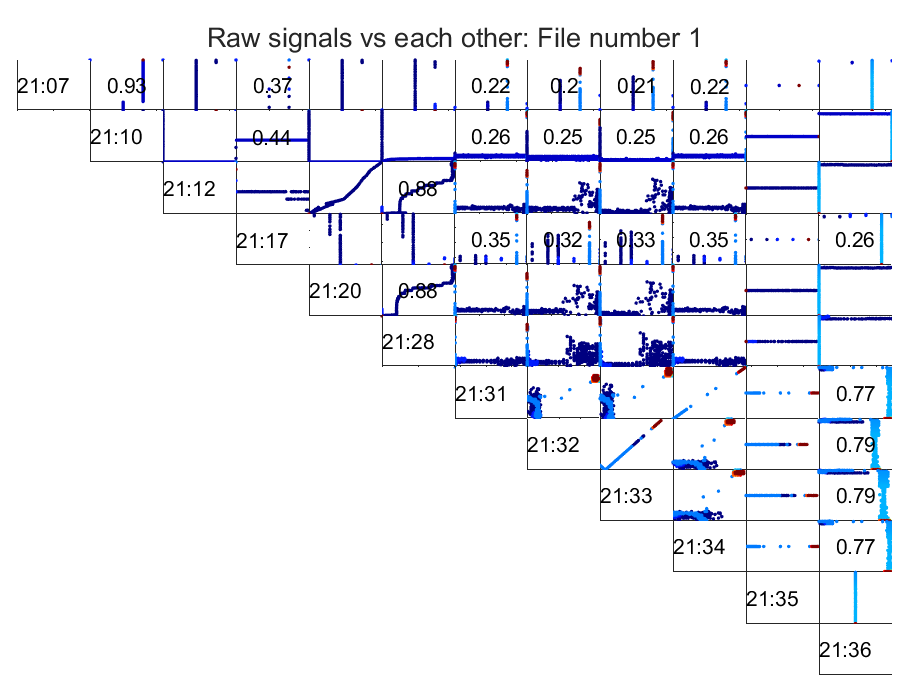
\includegraphics[width=\textwidth, height=\textheight, keepaspectratio]{figures/RawSignalCorrelationsFile1.eps}
    \caption{Plots of each signal vs every other signal R-square values between 0.2 and 0.9 printed on the plot}
    \label{fig:RawSignalCorrelationsFile1}
\end{figure}
Figure \ref{fig:RawSignalCorrelationsFile1} is somewhat linear and from Table \ref{correlationTable} has an R2 correlation value of 0.88.
\begin{figure}[H]
    \centering
    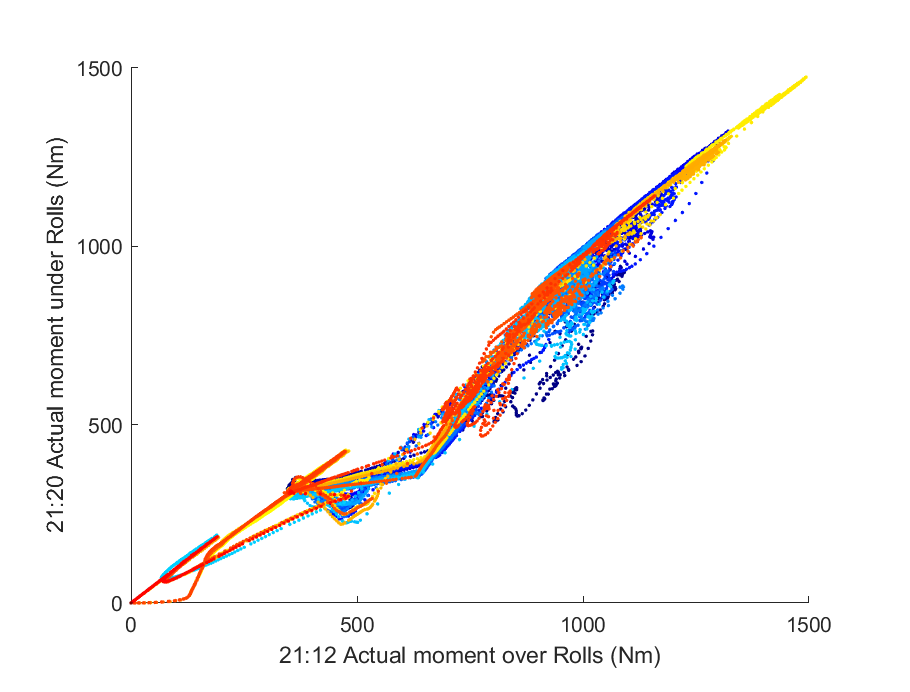
\includegraphics[width=\textwidth, height=\textheight, keepaspectratio]{figures/Signal21_12vSignal21_20.eps}
    \caption{Signal 21.12 vs Signal 21.20}
    \label{fig:Signal21_12vSignal21_20}
\end{figure}	
Figure \ref{fig:Signal21_20vSignal21_28} could be a non-linear relationship
\begin{figure}[H]
    \centering
    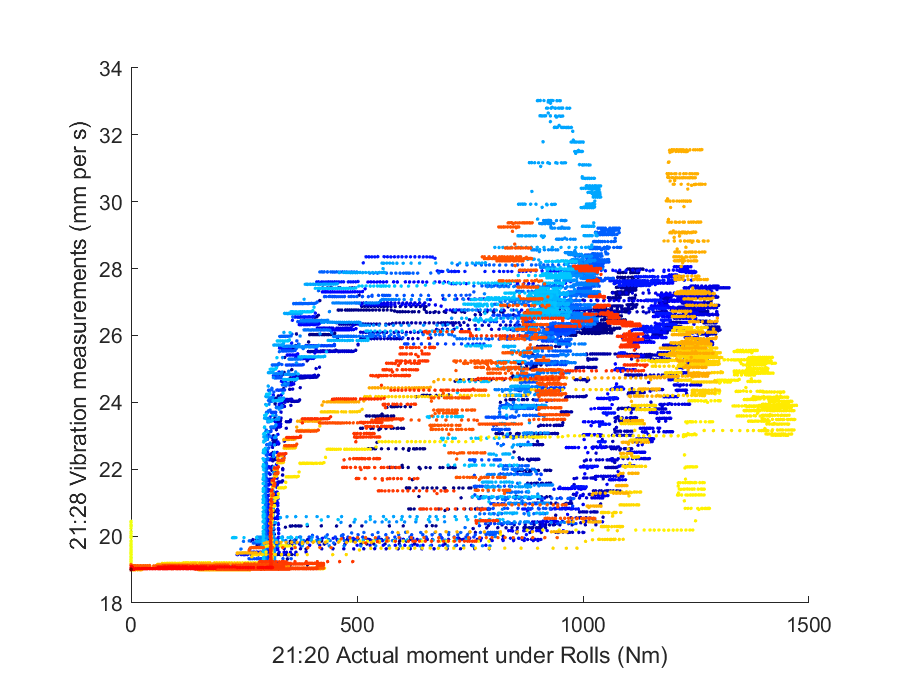
\includegraphics[width=\textwidth, height=\textheight, keepaspectratio]{figures/Signal21_20vSignal21_28.eps}
    \caption{Signal 21.20 vs 21.28}
    \label{fig:Signal21_20vSignal21_28}
\end{figure}	
	
\subsection{Pre-processing}
Figure \ref{fig:StateDetection} shows the windows that were identified from each file where the 21.20 signal was above the threshold. Two files, B\_30\_03 and B\_04\_04, contained no identified pulses. In total 240 pulses were identified. Some of these identified pulses were too short and thus believed to be false positives. Thus any pulse under 500 samples (1 second?) was removed from the data for the next stage leaving 224 pulses to extract features from.

\begin{figure}[H]
    \centering
    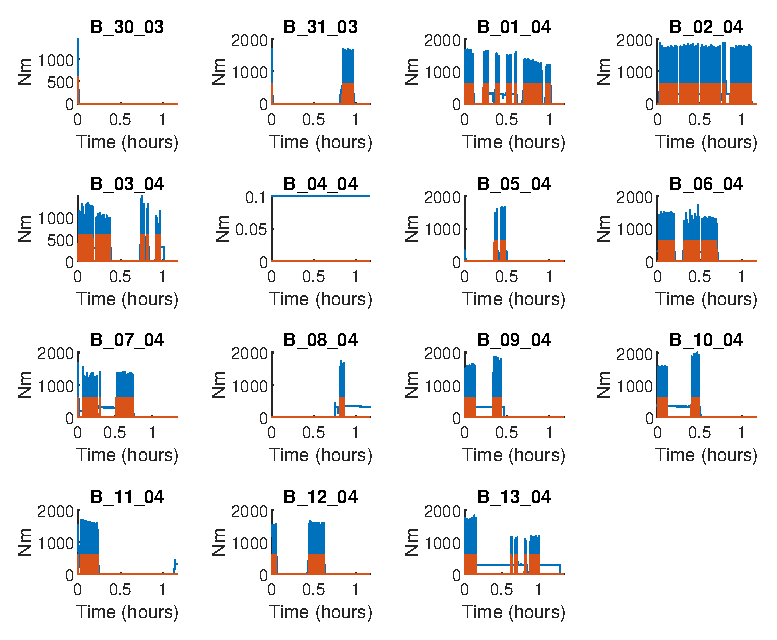
\includegraphics[width=\textwidth, height=\textheight, keepaspectratio]{figures/StateDetectionFig.eps}
    \caption{State detection signal vs 21:20 Actual moment under Rollers}
    \label{fig:StateDetection}
\end{figure}

Figure \ref{fig:StateDetectionFig_B_02_04} shows one of the plots from Figure \ref{fig:StateDetection} in greater detail. This particular file is the one with the highest number of pulses.
\begin{figure}[H]
    \centering
    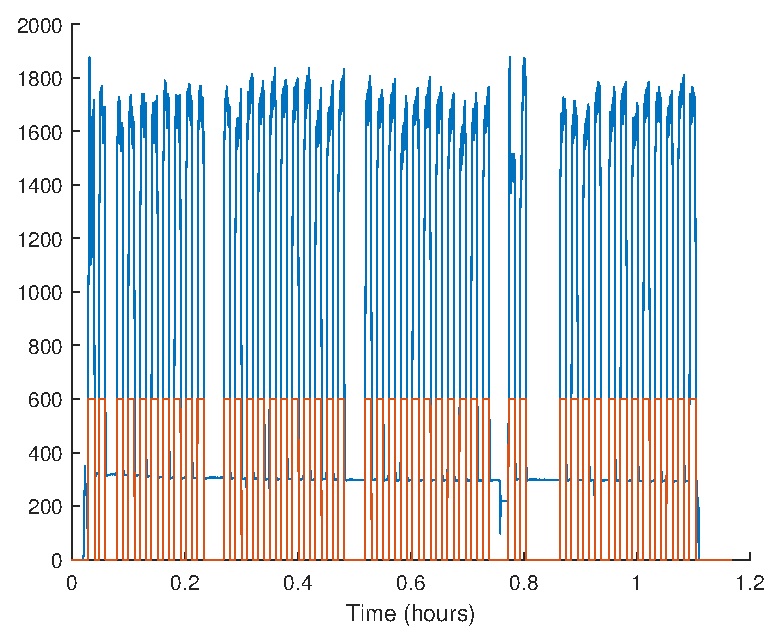
\includegraphics[width=\textwidth, height=\textheight, keepaspectratio]{figures/StateDetectionFig_B_02_04.eps}
    \caption{XXX}
    \label{fig:StateDetectionFig_B_02_04}
\end{figure}

Figure \ref{fig:IdentifiedPulses} show 
\begin{figure}[H]
    \centering
    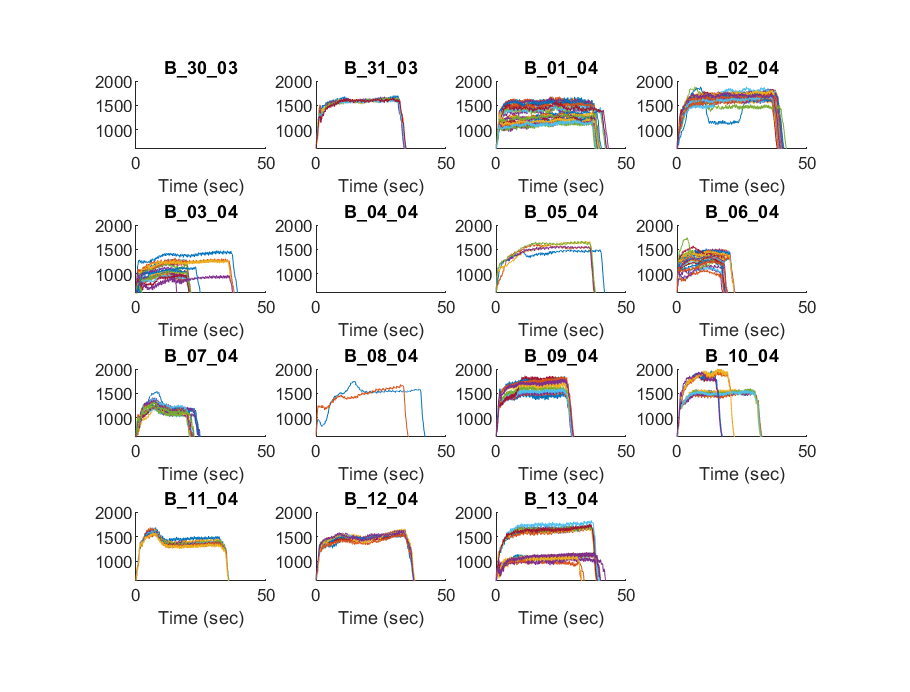
\includegraphics[width=\textwidth, height=\textheight, keepaspectratio]{figures/IdentifiedPulsesFig.eps}
    \caption{Identified pulses in each files for file}
    \label{fig:IdentifiedPulses}
\end{figure}

\subsection{Visual Observations}
Figure \ref{fig:SignalPulses} shows the signals for 225 pulses. Each sensor channel is plotted a different tile. 
\begin{figure}[H]
    \centering
    \includegraphics[width=\textwidth, height=\textheight, keepaspectratio]{figures/SignalPulses.eps}
    \caption{Signal pulses for 225 pulses on each of the 12 signal channels}
    \label{fig:SignalPulses}
\end{figure}

Signal 21.07 Angle over Rolls and 21.XX, 21.31, etc are fairly unexciting. They are just straight lines.
Where as signal XX.XX contains a lot of information.
21.35 is a constant signal so when we remove the mean all signals are exactly the same.

Figure \ref{fig:SignalPulse5} shows 
\begin{figure}[H]
    \centering
    \includegraphics[width=\textwidth, height=\textheight, keepaspectratio]{figures/SignalPulse5.eps}
    \caption{Signale 5 Pulses}
    \label{fig:SignalPulse5}
\end{figure}

%Figure \ref{fig:SignalTrace21.20} shows 21:20 Actual moment under Rolls (Nm)
%\begin{figure}[H]
%    \centering
%    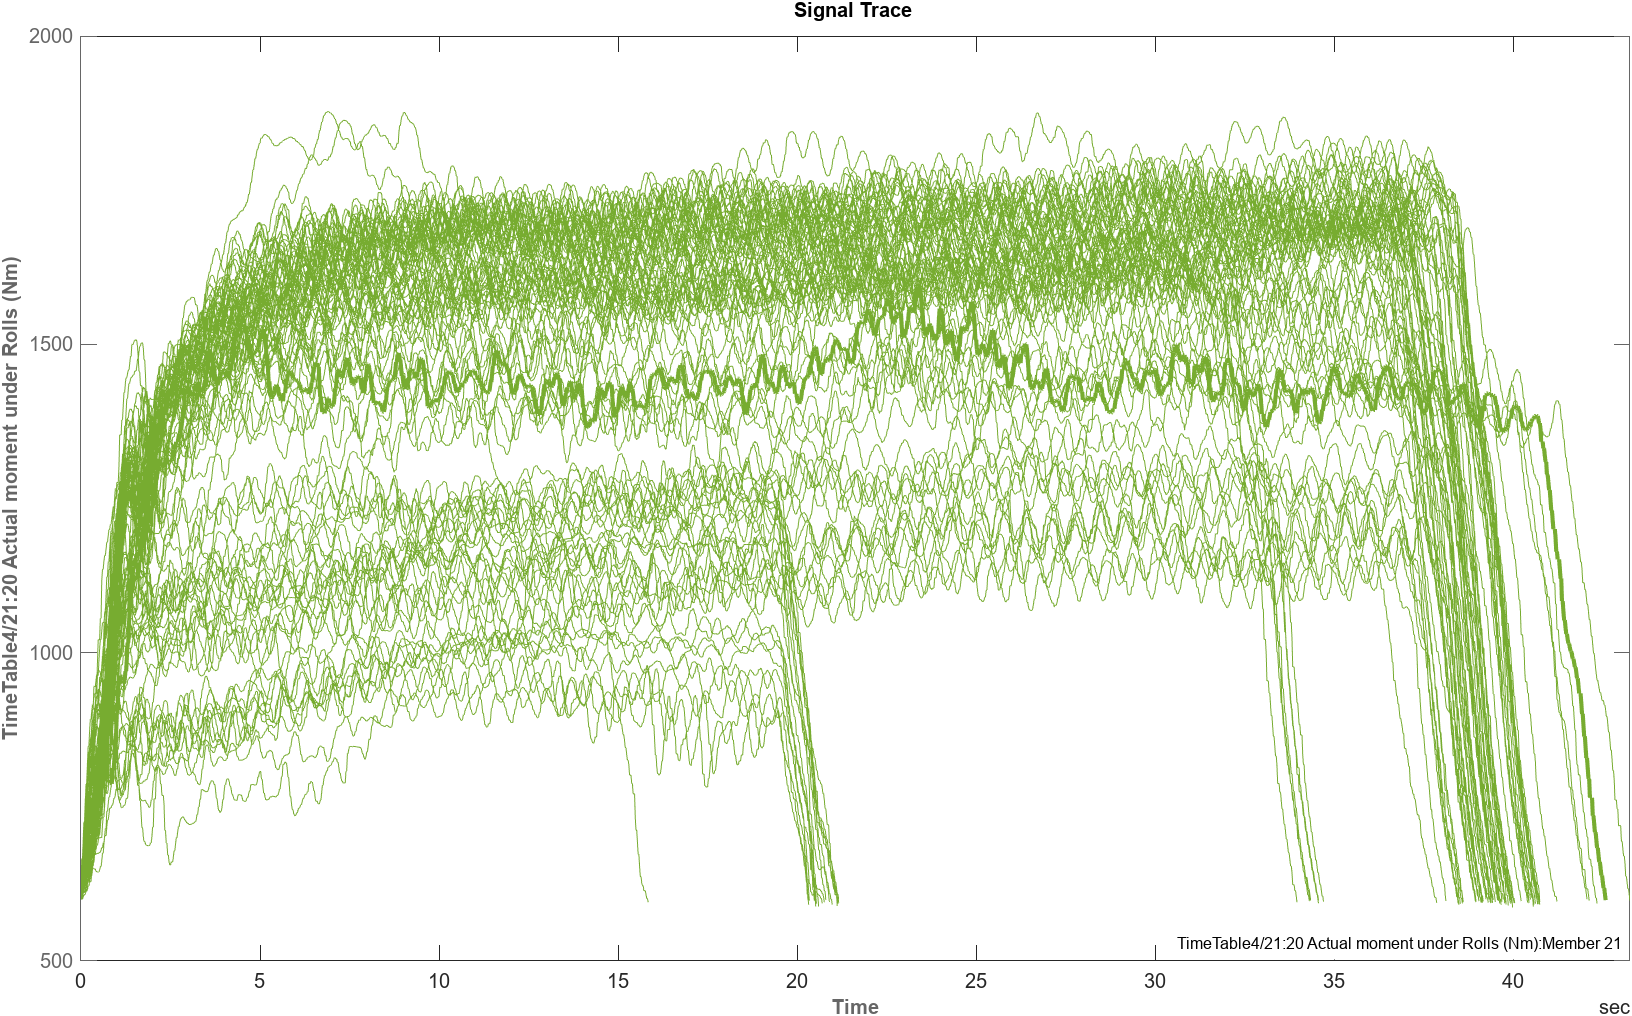
\includegraphics[width=\textwidth, height=\textheight, keepaspectratio]{figures/SignalTrace21.20.png}
%    \caption{Signal Trace 21.20}
%    \label{fig:SignalTrace21.20}
%\end{figure}

%Figure \ref{fig:SignalTrace21.12} shows ...
%\begin{figure}[H]
%    \centering
%    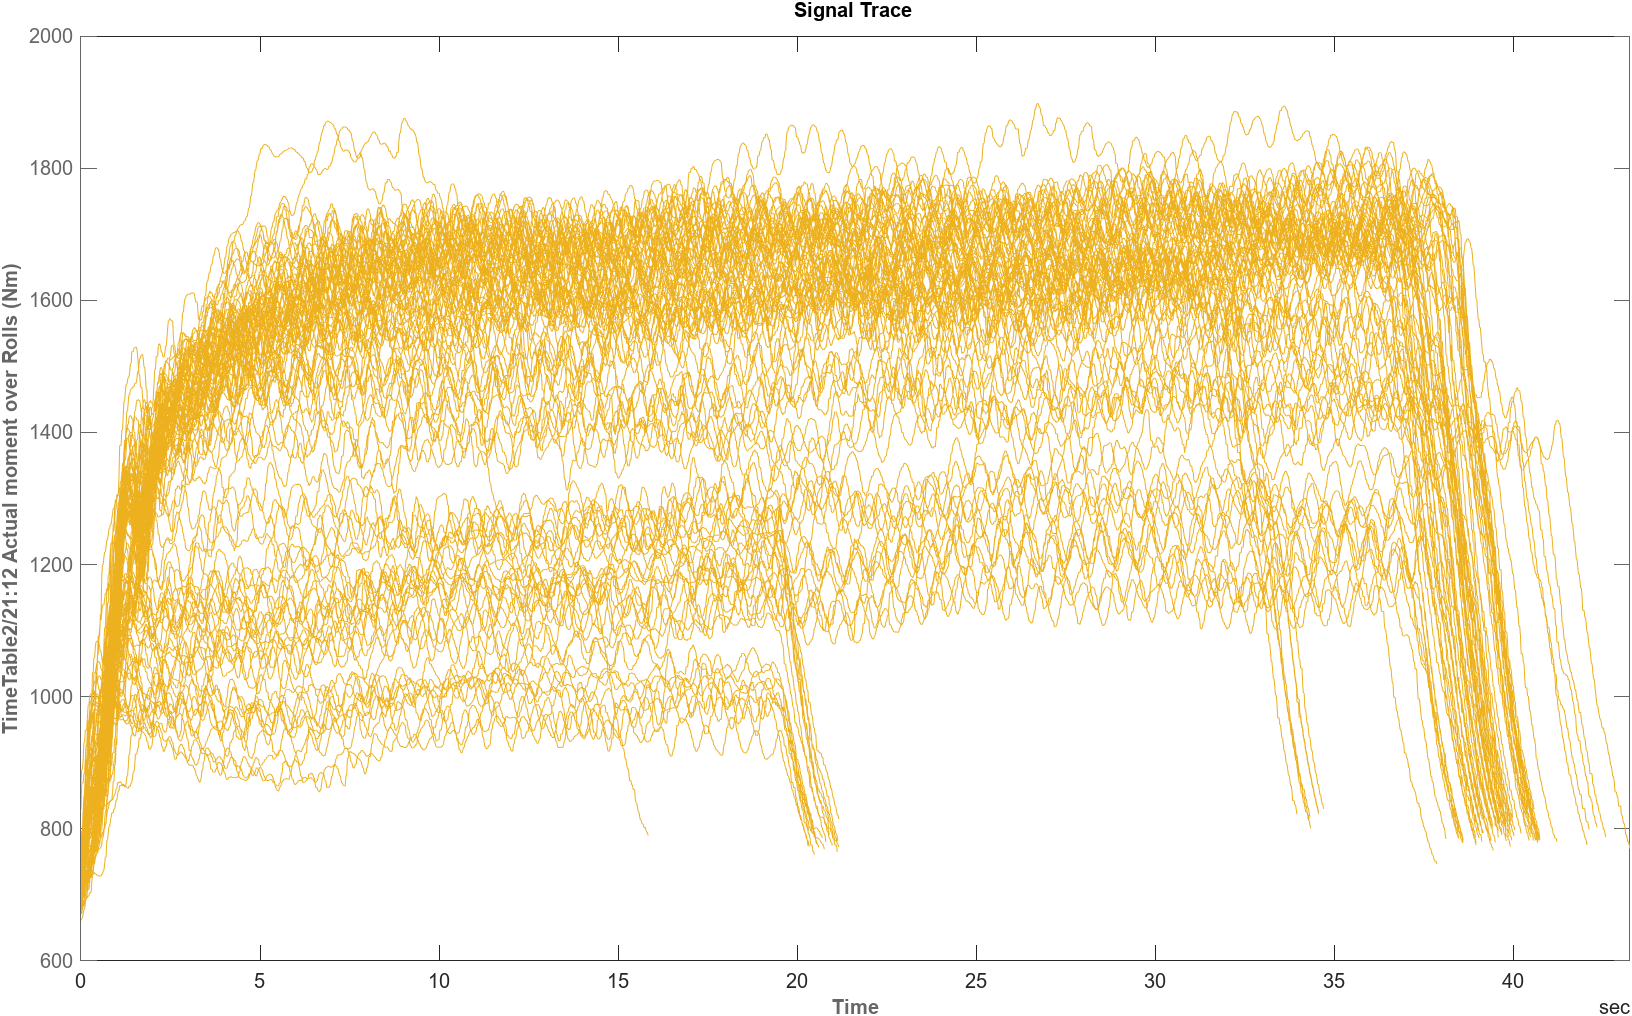
\includegraphics[width=\textwidth, height=\textheight, keepaspectratio]{figures/SignalTrace21.12.png}
%    \caption{Signal Trace 21.12}
%    \label{fig:SignalTrace21.12}
%\end{figure}

%Figure \ref{fig:SignalTrace21.28} shows ...
%\begin{figure}[H]
%    \centering
%    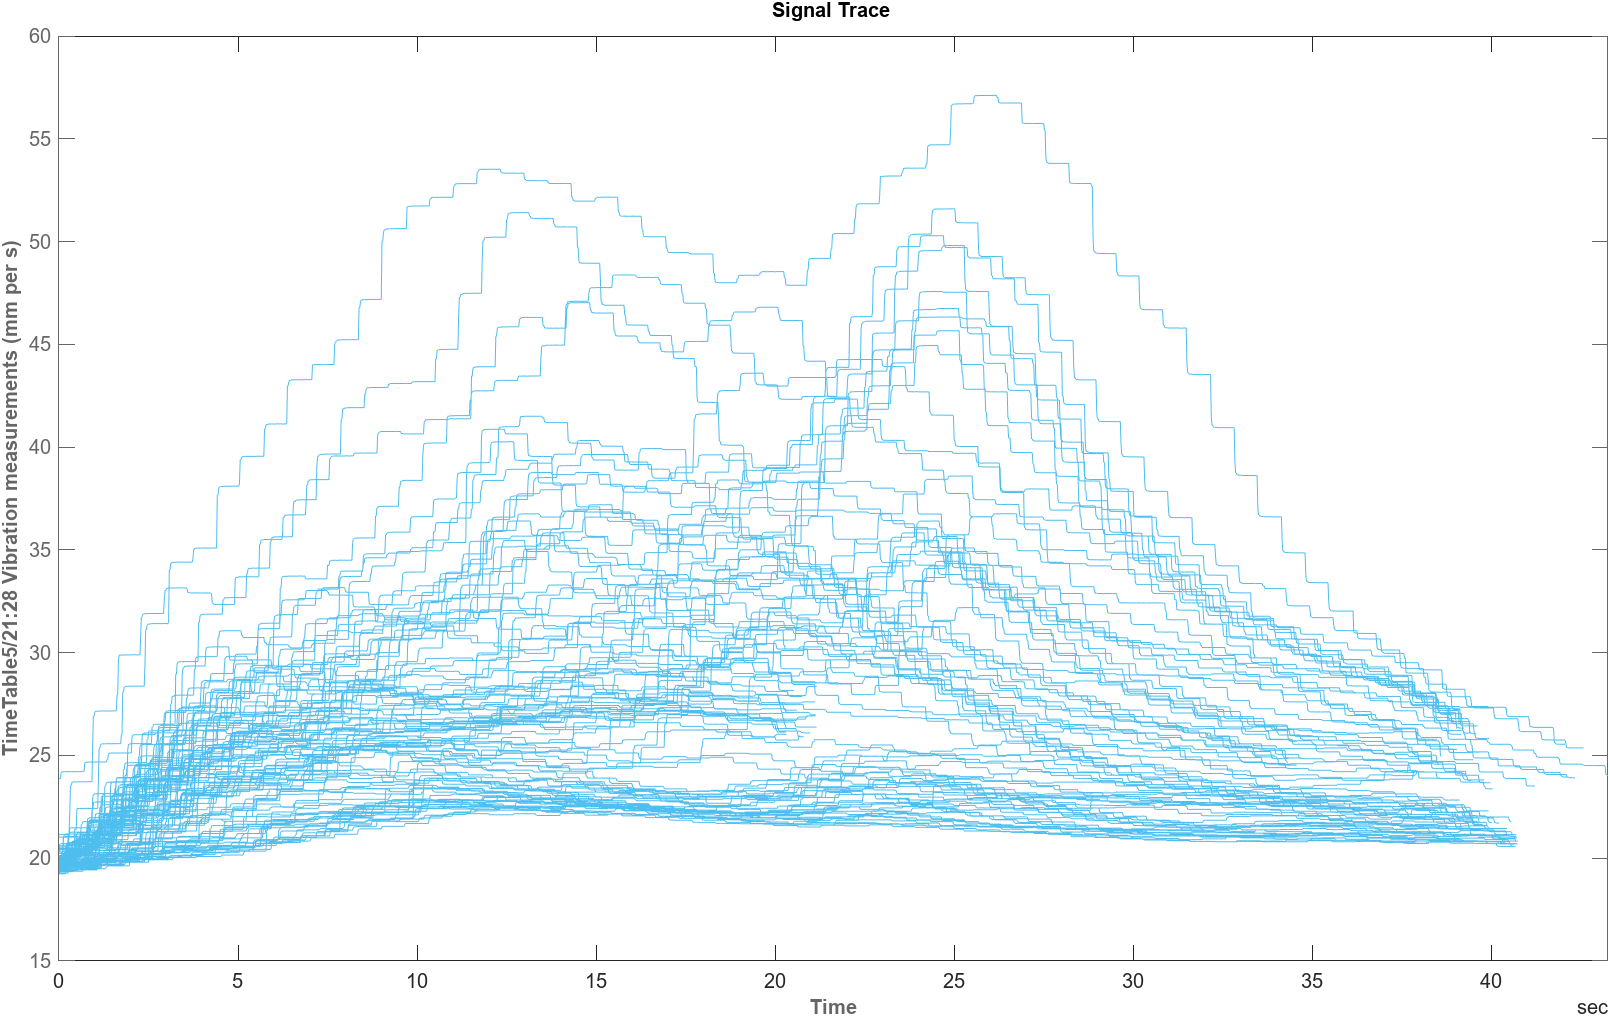
\includegraphics[width=\textwidth, height=\textheight, keepaspectratio]{figures/SignalTrace21.28.png}
%    \caption{Signal Trace 21.28}
%    \label{fig:SignalTrace21.28}
%\end{figure}

%Figure \ref{fig:SignalTrace21.07} shows 
%\begin{figure}[H]
%    \centering
%    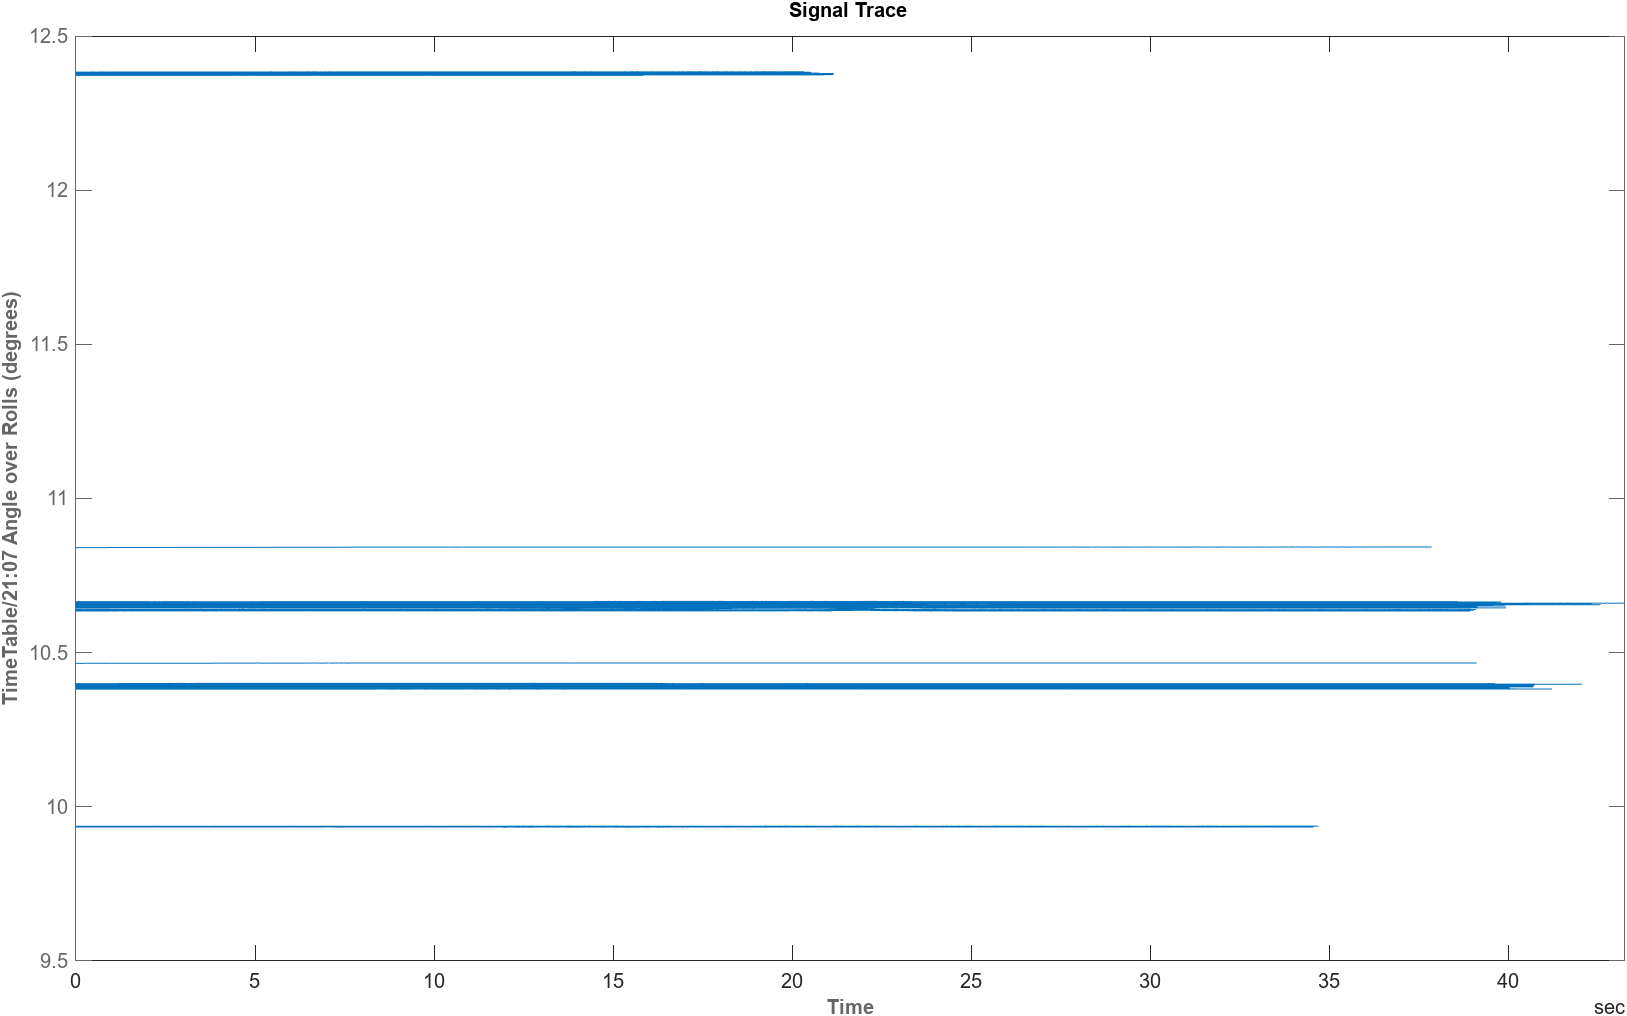
\includegraphics[width=\textwidth, height=\textheight, keepaspectratio]{figures/SignalTrace21.07.png}
%    \caption{Signal Trace 21.07}
%    \label{fig:SignalTrace21.07}
%\end{figure}

%Figure \ref{fig:SignalTrace21.35} shows ...
%\begin{figure}[H]
%    \centering
%    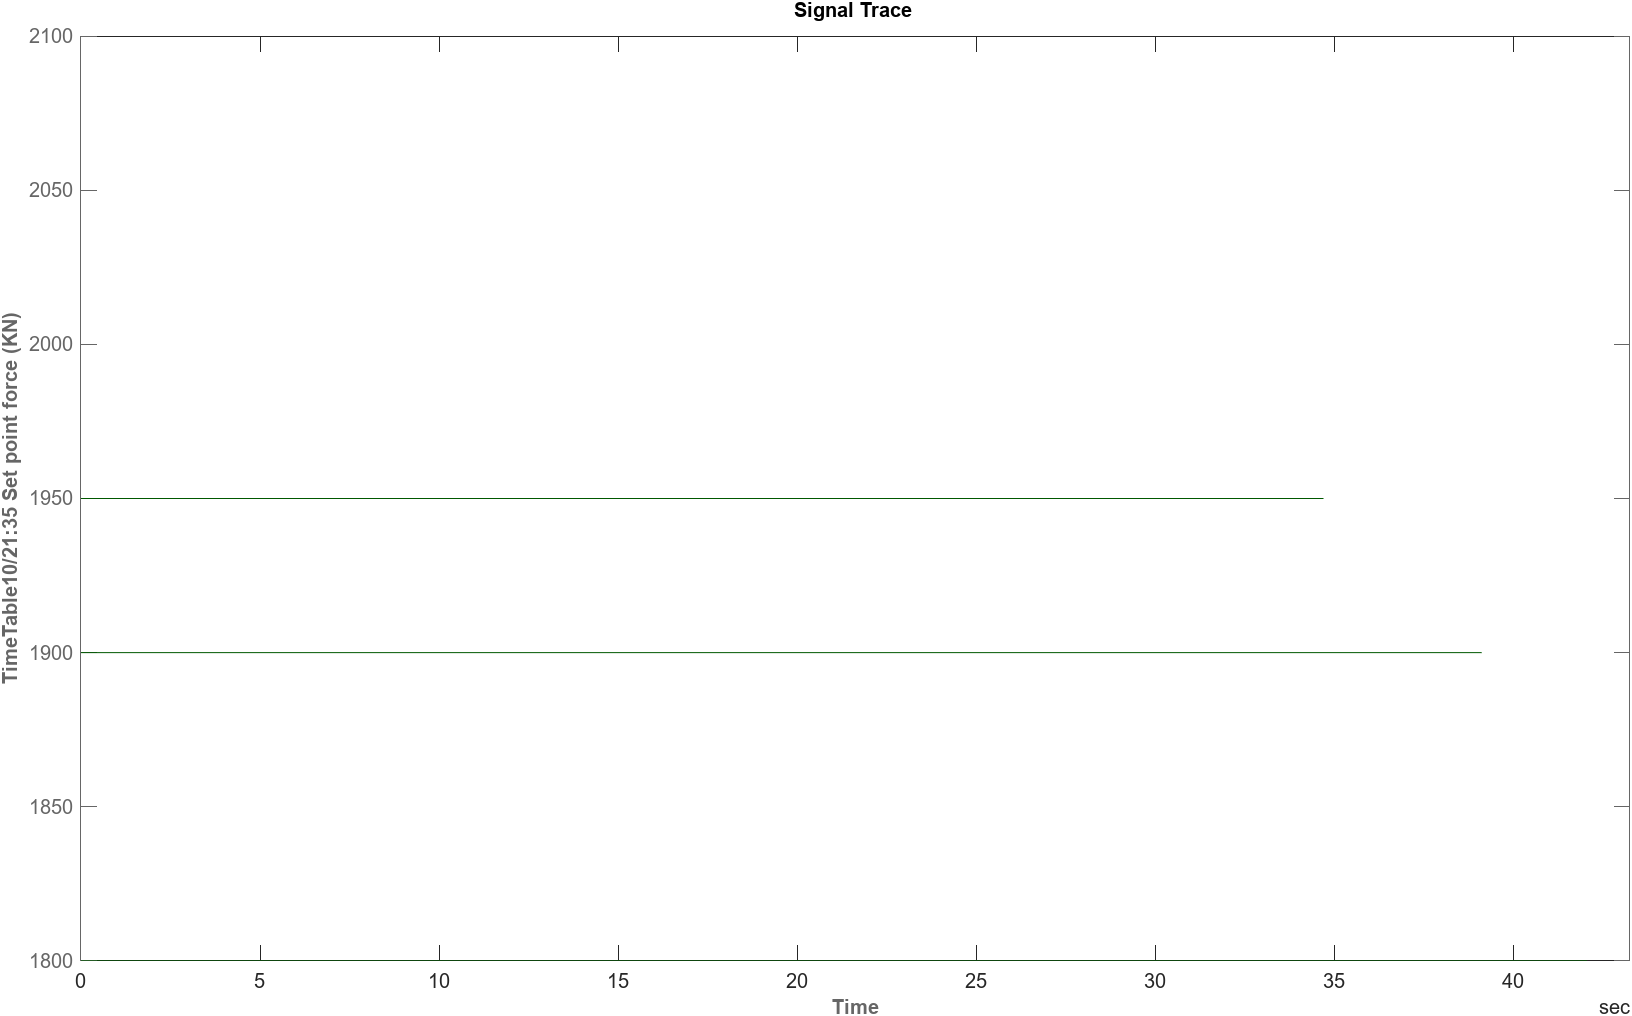
\includegraphics[width=\textwidth, height=\textheight, keepaspectratio]{figures/SignalTrace21.35.png}
%    \caption{Signal Trace 21.35}
%    \label{fig:SignalTrace21.35}
%\end{figure}

\subsection{Feature Extraction}

\subsubsection{Feature vs Feature}
Figure \ref{fig:FeatureVsFeatureSignal1} shows 
\begin{figure}[H]
    \centering
    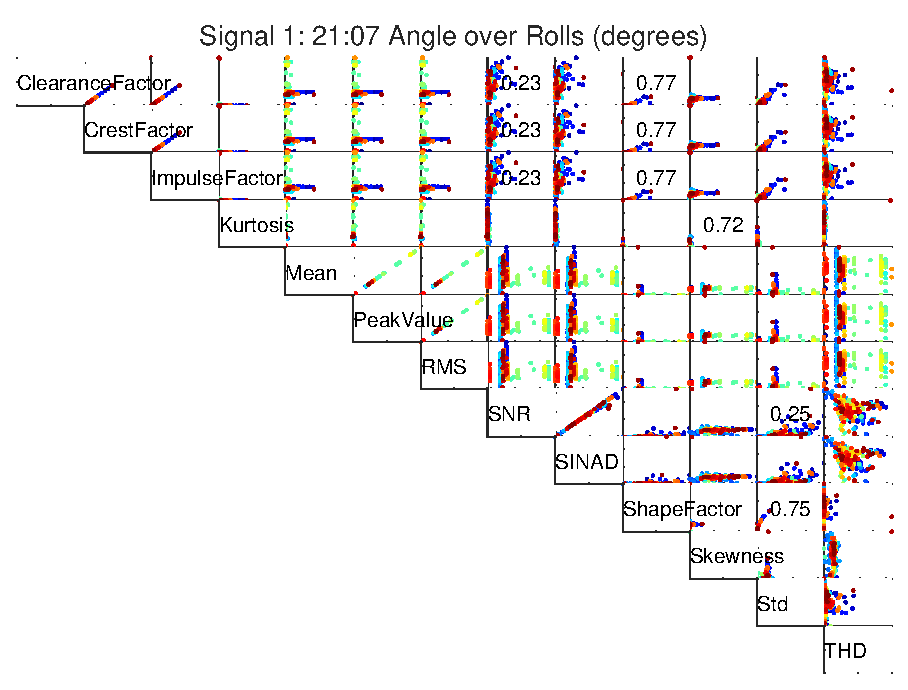
\includegraphics[width=\textwidth, height=\textheight, keepaspectratio]{figures/FeatureVsFeatureSignal1.eps}
    \caption{Feature Vs Feature for Signal 1 21.07}
    \label{fig:FeatureVsFeatureSignal1}
\end{figure}

\subsubsection{Signal vs Signal}
Figure \ref{fig:FeatureVsFeatureSignal1} shows 
\begin{figure}[H]
    \centering
    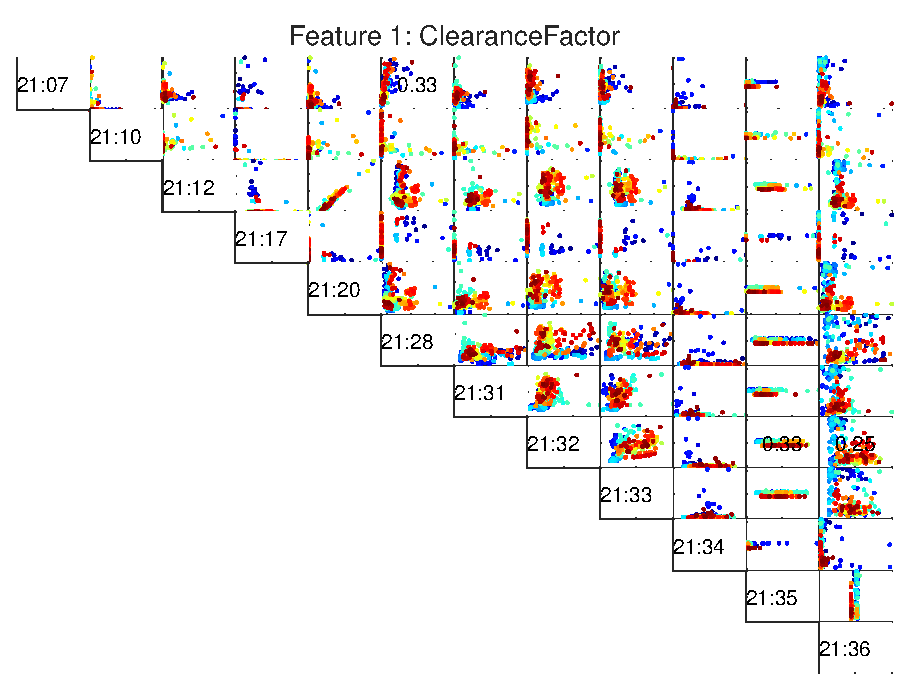
\includegraphics[width=\textwidth, height=\textheight, keepaspectratio]{figures/SignalVsSignalFeature1.eps}
    \caption{Signal Vs Signal for Feature 1}
    \label{fig:SignalVsSignalFeature1}
\end{figure}
\subsection{Linear Models}

\subsection{Multivariate models}

\clearpage 
\section{Conclusions}
One conclusion could be that "for future condition monitoring work we need to only focus on this data (might only be 10\%)".\\
Another conclusion could be that we need to go forward to doing this and that.\\
Conclusion could be what we say to the company or what we need.\\
Would temperature of something be good to monitor?\\
Worth doing an analysis based on different sizes
Ideally we would have data over the lifespan of a machine. The data we have right know, we don't know whether is is normal operating data. It could be right at the beginning of the lifecycle or could be just at the end of the machines lifecycle. A system that has been operating for a long period of time will undergo changes due to the natural wear of the system.
One conclusion might be just to discard all the signals with constant values.
\newpage
\section{Discussion} 
One of the next tasks should be to investigate apply unsupervised learning approaches to the signals highlighted in this project.
KNN or
K-means clustering approach.
Discuss results and put in context/comparison with references at the beginning. Future work.
\clearpage
\section{References} 
\printbibliography[heading=none] 
\clearpage  
\section{Appendix A - MATLAB Code}
\UseRawInputEncoding
\lstinputlisting[frame=single, numbers=left, style=Matlab-editor]{"./MATLAB Software/LoadRawData.m"}
\lstinputlisting[frame=single, numbers=left, style=Matlab-editor]{"./MATLAB Software/LoadFeatures.m"}
%\lstinputlisting[frame=single, numbers=left, style=Matlab-editor]{"./MATLAB Software/PreProcessData.m"}
\end{document}